\documentclass[12pt,a4paper]{article}
\usepackage{fontspec}
\defaultfontfeatures{Mapping=tex-text}
\usepackage{xunicode}
\usepackage{xltxtra}
%\setmainfont{???}

\makeatletter
\let\NAT@parse\undefined
\makeatother  %dovrebbe linkare citazioni e biblio, evitando che biblatex interferisca con hyperref

\usepackage{hyperref}
\usepackage{polyglossia}
\setdefaultlanguage{english}
\usepackage{amsmath}
\usepackage{amsfonts}
\usepackage{amssymb}
\usepackage{graphicx}
\usepackage{import}
\usepackage{pdfpages}
\usepackage[backend=bibtex, style=authoryear]{biblatex}
\addbibresource{bibliosempaper}
\usepackage{csquotes}
\usepackage{siunitx}
\usepackage{float}
\usepackage{caption}
\usepackage{xcolor}
\usepackage{glossaries}

\makenoidxglossaries

\newglossaryentry{sich verhalten}
{
    name=sich verhalten,
    description={to behave/act}
}


\newglossaryentry{sein}
{
    name=sein,
    description={to be}
}


\newglossaryentry{Anja war atemlos}
{
    name=Anja war atemlos,
    description={Anja was out of breath}
}


\newglossaryentry{Dennis war intelligent}
{
    name=Dennis war intelligent,
    description={Dennis was intelligent}
}


\newglossaryentry{Sophie verhielt sich betrunken}
{
    name=Sophie verhielt sich betrunken,
    description={Sophie acted drunk}
}


\newglossaryentry{Holger verhielt sich spanisch}
{
    name=Holger verhielt sich spanisch,
    description={Holger behaved Spanish}
}


\newglossaryentry{Alina wartete auf die Ergebnisse}
{
    name=Alina wartete auf die Ergebnisse,
    description={Alina was waiting for the results}
}



\sisetup{
  round-mode = places, % to round the numbers
  round-precision = 2, % to have two numbers after the decimal point
}
\usepackage[left=2cm,right=2cm,top=2cm,bottom=2cm]{geometry}
\author{Federica Mazzucco}
\title{Stage-level and Individual-level Adjectives: acceptability in relation to neutral verbs and control-intention verbs}
\begin{document}

\maketitle
\vspace{3.5cm}
\tableofcontents
\newpage
\section{Background}

In order to understand the goal of the study, it is first necessary to look into the definitions of stage-level and individual-level properties. \citeauthor{Kratzer1995} offers an easy to grasp definition, if a bit simplistic:

\begin{quote}
"That I am sitting on this chair is a very transitive property of mine. That I have brown hair is not. The first property is a \textit{stage-level property} [...], the second property is an \textit{individual-level property}."
 \parencite{Kratzer1995}
\end{quote}

By sticking to this definition, we might be tempted to tie the stage-level property to something extremely short and volatile, like being sat down, being focused on a videogame or happy for scoring a goal. However, we will also encounter examples like the one below:

\begin{enumerate}
\item Jake was disabled (for his whole life)
\item Jake was disabled (but he regained full mobility through physical therapy)
\end{enumerate}

Like many other adjectives, "disabled" can be used as both individual-level and stage-level adjective. In the latter case, it is often hard to understand the transient connotation expressed by the adjective. \citeauthor{Carlson1977} tackles this issue by making a distinction in the recipient of the adjective:


\begin{quote}
"Suppose we take an individual, Jake, and look at him as being composed of a set of Jake-stages, or temporally-bounded portions of Jake's existence. There is more to Jake, however, than a set of stages. There is whatever it is that ties all these stages together to make them stages of the same thing. Let us call this whatever-it-is the individual Jake. Those predicates we have been calling "states" then are not predicated of individuals, but of stages of individuals; and those we have been calling "properties" [...] are predicated of the individual  or the thing that ties all the stages together" \parencite{Carlson1977} 
\end{quote}


By this, \citeauthor{Carlson1977} means to warn us about the difference of the subject of the stage-level predicate or, in our case, the subject that the adjective refers to: it consists of only a stage of the individual, not the individual itself. This specific version of the subject can persist for an indefinite amount of time, even for very long period, but is still ultimately temporally-bound; the individual itself and its characteristics are instead not temporally connotated.

We understand that the stage-level adjective is not tied to the length of the property it expresses, but rather to the fact that said property can begin and finish. The adjective used in the example above is still a stage-level property, even though it can take up a very long portion of the individual's existence.\\

The nature of control or intention verbs is also relevant to this study. These verbs express a degree of deontic modality, that is the modality concerning the obligation and possibility, also in relation to the speaker's intention \parencite{simpson1993}, in its subcategory of volitive modality. In particular, the verb \textit{\gls{sich verhalten}} (to behave/act), which recurs in the experiment, seems to fall into the category of Intention-to-Action verbs, described by \parencite{Khudairi2015} %Hasen
 as "the intentional pursuit, by the agent, of a course of action". 

On the other hand, a neutral verb does not express any degree of modality. In our case, the neutral verb used is \textit{\gls{sein}} (to be). This particular verb can assume various types of modality when used as an auxiliary verb or as part of a complex verbal construction, e.g. \textit{to be able to}, but it will not be the case in the present study.\\

The experiment illustrated in the following sections will deal both the verb types above introduced, and their acceptability in relation to stage-level adjectives and individual-level adjectives. Two contrasting theories will be tested:

\begin{itemize}
\item \textbf{Theory A}: Both verb types will be judged equally well with both adjective types.
\item \textbf{Theory B}: The verb \textit{\gls{sich verhalten}} (to behave/act) will be incompatible with the individual-level adjectives.
\end{itemize}

The following sections illustrate the experiment created to test the two theses. 


\section{Methods}

\subsection{Design}

The experiment was designed as a rating task, and it uses a 1 to 7 Likert scale. The stimuli were declarative sentences in the past simple tense, containing either a stage-level or an individual level adjective, and a neutral verb or a verb expressing control or intention. While the adjectives where 60 in total, it was decided to only include two verbs:

\begin{itemize}
\item \textit{\gls{sein}} (to be), as the neutral verb,
\item \textit{\gls{sich verhalten}} (to behave/act), as the control/intention verb.
\end{itemize}

The experimenters thus obtained 4 conditions, plus a control category, as illustrated in \textcolor{cyan}{Table \ref{Table 1}}.\\


\begin{table}[h]
\captionsetup{font=scriptsize}
\begin{tabular}{||l|l|l|l||}
\hline
\textbf{Condition} & \textbf{Adjective} & \textbf{Verb} & \textbf{Example}\\
\hline \hline
1 & Stage-level & \gls{sein} & \gls{Anja war atemlos}\\
\hline
2 & Individual-level & \gls{sein} & \gls{Dennis war intelligent} \\
\hline
3 & Stage-level & \gls{sich verhalten} & \gls{Sophie verhielt sich betrunken} \\
\hline
4 & Individual-level & \gls{sich verhalten} & \gls{Holger verhielt sich spanisch}\\
\hline
100 & Control adjective & Control verb & \gls{Alina wartete auf die Ergebnisse} \\
\hline
\end{tabular}
\caption{Structure and examples for each condition.}
\label{Table 1}
\end{table}


The stimuli were divided into 4 equivalent lists. Each list was given to 10 people, and contains either 7 or 8 sentences for each condition, as illustrated by \textcolor{cyan}{Table \ref{Table 2}}.


\begin{table}[h]
\captionsetup{font=scriptsize}
\begin{tabular}{||l|l|l|l|l||}
\hline
\textbf{List number} & \textbf{Condition 1} & \textbf{Condition 2} & \textbf{Condition 3} & \textbf{Condition 4}\\
\hline \hline

List 1 & 8 & 7 & 7 & 8\\

List 2 & 8 & 8 & 7 & 7\\

List 3 & 7 & 8 & 8 & 7\\

List 4 & 7 & 7 & 8 & 8\\

\hline
\end{tabular}
\caption{Number of sentences of relevant conditions in the lists.}
\label{Table 2}
\end{table}

A similar experiment design can be found at the link \textcolor{cyan}{\url{https://www.lingexp.uni-tuebingen.de/OnExp2/onexp.php?status=new&username=PAnna&experimentname=Persian}}. 

\subsection{Participants}

The participants were 40 students of the University of Tubingen, who took part in the study remotely. They were automatically assigned a code, and they received a payment of 5€ if they completed the study and sent their code to the organizers. The participants' age ranged from 18 to 30. In the group, 24 students identified as female, 12 as male and 4 as other. Each of them was presented with 30 of the target sentences (Conditions 1 to 4), as well as 100 control sentences.

Due to a mistake in one of the participant's data, one person had to be removed from the database. As a consequence, the results are based on the answers of 39 participants.

\subsection{Procedure}

The experiment took place online, through a link provided by the University of Tubingen. The participants were instructed to click on the link, and read the initial instructions. They were asked to answer a few personal questions, concerning their native language (German and/or other), and the specific variant of German they speak, corresponding to which Federal State. Data were also collected about their gender, age and handedness. Any personal data collected is to remain anonymous and can only be used for statistical purposes.

The students were asked to read the sentences and rate their naturalness from 1 to 7 (1 being the lowest level of naturalness). They had to read quickly, but still give themselves the time to understand the sentence, and they were recommended to simply use their intuition in the rating phase.
Two example sentences were provided, one very natural, the other very unnatural, in order to make them familiar with the task.

The estimated time to complete the experiment was 45 minutes. None of the participant was aware of the purpose of the experiment, but at the end of their contribution they were provided a short explanation on the topic of the study.

\subsection{Predictions}

We can expect strongly diverging results according to which thesis will prove to be correct.\\

In case of theory 1 being right, we expect the results to show equal high ratings for all the conditions, demonstrating that both verb types can be paired equally well with stage-level and individual-level adjectives.

However, if theory 2 will prove to be right, we can expect the results to vary in condition 4, which pairs a control/intention verb with an individual-level adjective, compared to the other three conditions. Theory 2 indeed hypothesizes that the two paired factors will receive significantly lower ratings, as they will sound unnatural to the participants.

\section{Results and Discussion}

The analysis of the results shows a clear difference of ratings in the fourth condition, the one pairing a control/intention verb with an individual-level adjective. \textcolor{cyan}{Figure \ref{Figure 1}} shows the amount of ratings corresponding to each point in the scale for all relevant conditions. In conditions 1, 2 and 3, more than half of the ratings were >= 5. On the other hand, condition 4 counts 205 ratings that are <=3, whith only two rating 6, and no ratings being assigned corresponding to the higher point in the scale.


\begin{figure}[h]
\centering
\captionsetup{font=scriptsize}
  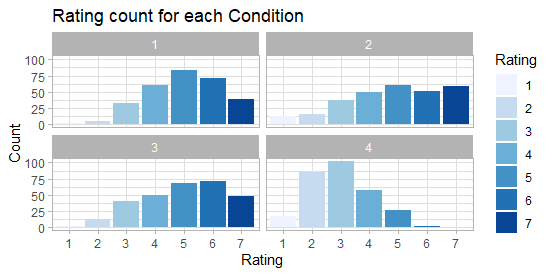
\includegraphics[width=1\textwidth]{Rating_count.PNG}
  \caption{Number of ratings for each condition, in each point of the Likert scale.}
  \label{Figure 1}
\end{figure}

According to the data collected, the experiment seems to favour theory 2: a control/intention verb paired with an individual-level adjective will generally produce unnatural-sounding sentences. It is already established that the acceptability of individual-level adjectives indeed varies in relation to many factors, one of them being the aspect of the preceding verb \parencite{husband2006} and this experiment only confirms the high variability in how acceptable these particular adjective are, compared to stage-level adjectives.


However, a question arises: Are the data to be trusted? In case of a significantly higher standard variation in one of the conditions, the mean for this specific condition will be less accurate and potentially misleading. For example, suppose the ratings of a condition fall exclusively on point 1 and 7 of the Likert scale (the two extremes). In this case, the mean rating will be 4, but it will not in any way depict the actual behaviour of the majority of the participants.

To prove the accuracy of our results, we can look at \textcolor{cyan}{Figure \ref{Figure 2}}. 

\begin{figure}[h]
\centering
\captionsetup{font=scriptsize}
  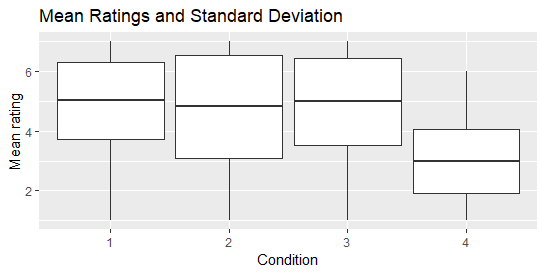
\includegraphics[width=1\textwidth]{MeanRat.PNG}
  \caption{The mean ratings correspond to the line dividing the boxes, while the vertical extension of the plot highlights the standard variations of the results.}
  \label{Figure 2}
\end{figure}

Here we can see how the standard deviations never exceed 1.5 points in te scale. Moreover, the mean rating never falls far from the rating assigned by the majority of the participants: for conditions 1, 2 and 4, the mean rating perfectly matches the point in the scale most chosen by the participants; while in condition 3 the mean rating only differs of 1 point from the actual preferred choice. To sum up, the results can be considered as reasonably accurate.

\vspace{2cm}

\printnoidxglossaries

\newpage

\printbibliography

\newpage

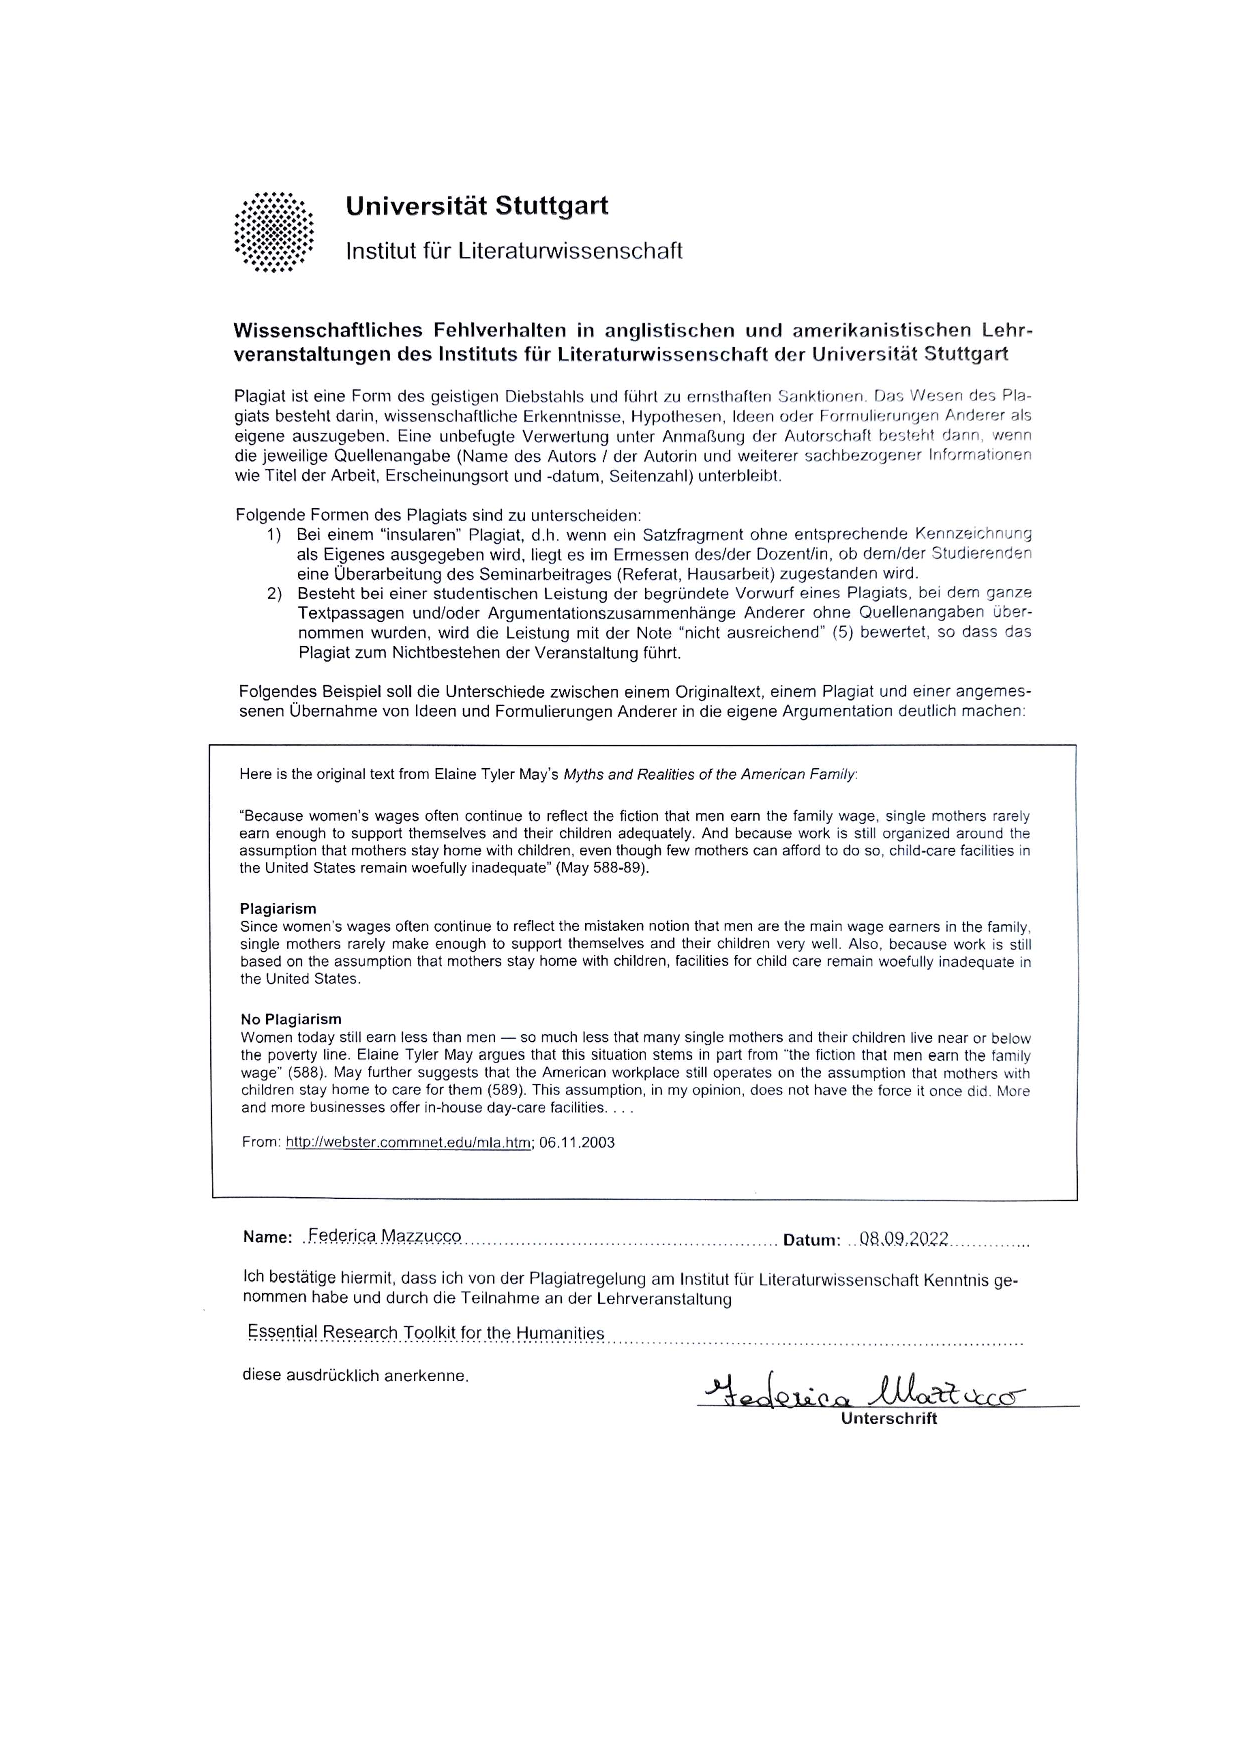
\includepdf{noplagiarism.pdf}

\end{document}